%% 
%% Copyright 2007-2024 Elsevier Ltd
%% 
%% This file is part of the 'Elsarticle Bundle'.
%% ---------------------------------------------
%% 
%% It may be distributed under the conditions of the LaTeX Project Public
%% License, either version 1.3 of this license or (at your option) any
%% later version.  The latest version of this license is in
%%    http://www.latex-project.org/lppl.txt
%% and version 1.3 or later is part of all distributions of LaTeX
%% version 1999/12/01 or later.
%% 
%% The list of all files belonging to the 'Elsarticle Bundle' is
%% given in the file `manifest.txt'.
%% 
%% Template article for Elsevier's document class `elsarticle'
%% with harvard style bibliographic references

\documentclass[preprint,12pt,authoryear]{elsarticle}

%% Use the option review to obtain double line spacing
%% \documentclass[authoryear,preprint,review,12pt]{elsarticle}

%% Use the options 1p,twocolumn; 3p; 3p,twocolumn; 5p; or 5p,twocolumn
%% for a journal layout:
%% \documentclass[final,1p,times,authoryear]{elsarticle}
%% \documentclass[final,1p,times,twocolumn,authoryear]{elsarticle}
%% \documentclass[final,3p,times,authoryear]{elsarticle}
%% \documentclass[final,3p,times,twocolumn,authoryear]{elsarticle}
%% \documentclass[final,5p,times,authoryear]{elsarticle}
%% \documentclass[final,5p,times,twocolumn,authoryear]{elsarticle}

%% For including figures, graphicx.sty has been loaded in
%% elsarticle.cls. If you prefer to use the old commands
%% please give \usepackage{epsfig}

%% The amssymb package provides various useful mathematical symbols
\usepackage{amssymb}
%% The amsmath package provides various useful equation environments.
\usepackage{amsmath}
\usepackage{textcomp}
\usepackage{rotating}  % Enables landscape floats (sidewaystable)
\usepackage{tabularx}  % For text wrapping
\usepackage{booktabs}  % For clean publication rules
\usepackage{array}
\usepackage{url}
%% The amsthm package provides extended theorem environments
%% \usepackage{amsthm}

%% The lineno packages adds line numbers. Start line numbering with
%% \begin{linenumbers}, end it with \end{linenumbers}. Or switch it on
%% for the whole article with \linenumbers.
%% \usepackage{lineno}

\journal{International Journal of Applied Earth Observation and Geoinformation}


\begin{document}

\begin{frontmatter}

%% Title, authors and addresses

%% use the tnoteref command within \title for footnotes;
%% use the tnotetext command for theassociated footnote;
%% use the fnref command within \author or \affiliation for footnotes;
%% use the fntext command for theassociated footnote;
%% use the corref command within \author for corresponding author footnotes;
%% use the cortext command for theassociated footnote;
%% use the ead command for the email address,
%% and the form \ead[url] for the home page:
%% \title{Title\tnoteref{label1}}
%% \tnotetext[label1]{}
%% \author{Name\corref{cor1}\fnref{label2}}
%% \ead{email address}
%% \ead[url]{home page}
%% \fntext[label2]{}
%% \cortext[cor1]{}
%% \affiliation{organization={},
%%            addressline={}, 
%%            city={},
%%            postcode={}, 
%%            state={},
%%            country={}}
%% \fntext[label3]{}

\title{FARMWISE-API: A Comprehensive Framework for Agricultural Data Integration} %% Article title

%% use optional labels to link authors explicitly to addresses:
%% \author[label1,label2]{}
%% \affiliation[label1]{organization={},
%%             addressline={},
%%             city={},
%%             postcode={},
%%             state={},
%%             country={}}
%%
%% \affiliation[label2]{organization={},
%%             addressline={},
%%             city={},
%%             postcode={},
%%             state={},
%%             country={}}

\author[label1]{Kamil Smolak} %% Author name
\author[label1]{Dominik Teodorczyk}
\author[label2]{Jakub Misiewicz}
\author[label3]{Marc Laurencelle}
\author[label2]{Wiesław Fiałkiewicz}
\author[label4,label5]{Arkadiusz Głogowski}
%% Author affiliation
\affiliation[label1]{organization={Institute of Geodesy and Geoinformatics, Wrocław University of Environmental and Life Sciences},%Department and Organization
            addressline={Norwida 25}, 
            city={Wrocław},
            postcode={50-375}, 
            state={},
            country={Poland}}
\affiliation[label2]{organization={Institute of Environmental Engineering, Wrocław University of Environmental and Life Sciences},%Department and Organization
            addressline={Norwida 25}, 
            city={Wrocław},
            postcode={50-375}, 
            state={},
            country={Poland}}      
\affiliation[label3]{organization={French Geological Survey, Bureau de recherches géologiques et minières},%Department and Organization
            addressline={3 avenue Claude-Guillemin}, 
            city={Orléans},
            postcode={45000}, 
            state={},
            country={France}} 
\affiliation[label4]{organization={Hydrogeology, Department of Environmental Sciences, University of Basel},%Department and Organization
            addressline={Bernoullistrasse 30/32}, 
            city={Basel},
            postcode={4056}, 
            state={},
            country={Switzerland}}    
\affiliation[label5]{organization={Department of Environmental Protection and Development, Wrocław University of Environmental and Life Sciences},%Department and Organization
            addressline={3 avenue Claude-Guillemin}, 
            city={Orléans},
            postcode={45000}, 
            state={},
            country={France}}
%% Abstract
\begin{abstract}
%% Text of abstract
The European agricultural sector faces an acute challenge of digital data fragmentation, where valuable environmental, meteorological, and hydrological datasets remain siloed across heterogeneous, non-interoperable systems. This fragmentation severely limits the development of evidence-based decision support tools essential for sustainable agriculture. Here we present FARMWISE-API, an open-source Python framework that addresses this problem through a unified data integration architecture. The system implements an adapter pattern to dynamically query 19 data sources (26 datasets) spanning meteorological, hydrological, soil, land-cover, groundwater and farm economic variables across Europe. A systematic bibliometric analysis of 34,531 agricultural publications (2001–2026) from Scopus is presented to contextualize the urgency of data integration: only 43.7\% of publications contain dataset-related content, approximately one-third lack spatial reference information, and despite a statistically significant structural increase in Open Access publishing following the DORA (2012) and FAIR (2016) initiatives—confirmed by Chow breakpoint tests (p < 0.001)—more than 50\% of publications remain behind paywalls. The FARMWISE-API framework resolves data heterogeneity through a hierarchical S2Cell spatial indexing system (Google S2 Geometry library), enabling seamless spatial harmonization across point-based and grid-based sources at user-defined resolutions. The dispatcher mechanism performs triple coverage checking—spatial, temporal, and thematic—before issuing any network request, minimizing unnecessary API calls. Results are returned as standardized pandas DataFrames with associated metadata. An interactive Folium-based visualization module generates standalone HTML maps supporting both raw and spatially interpolated displays. Comparative analysis against existing platforms (Copernicus, WISE, openEO, Weenat, Agdatahub, FaST) demonstrates that FARMWISE-API occupies a distinct niche as a fusion-oriented integration layer for researchers and decision-support developers. FARMWISE-API thus provides the foundational data infrastructure needed for the next generation of precision agriculture applications, directly supporting the objectives of the Common European Agricultural Data Space.
\end{abstract}

%%Graphical abstract
\begin{graphicalabstract}
%\includegraphics{grabs}
%abstract for fun TO BE CHANGED
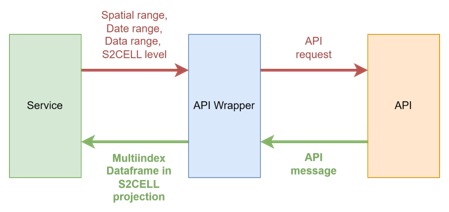
\includegraphics[width=\linewidth]{figs/obrazek_dominika.png}
\end{graphicalabstract}

%%Research highlights
\begin{highlights}
\item FARMWISE-API framework as a tool that help resolving data heterogeneity in agriculture data 
\item FARMWISE-API framework integrates meteorological, hydrological, soil, land-cover, groundwater and farm economic data
\item Based on a review of 34,531 publications regarding agricultural datasets (2001-2026) at Scopus more than 50\% of publications remain behind paywalls
\item 43.7\% of reviewed publications on agricultural data collection contain trackable dataset-related content
\end{highlights}

%% Keywords
\begin{keyword}
%% keywords here, in the form: keyword \sep keyword
Agriculture \sep data fragmentation \sep data integration \sep Open Access datasets \sep Decision support systems \sep Geospatial data harmonization
%% PACS codes here, in the form: \PACS code \sep code

%% MSC codes here, in the form: \MSC code \sep code
%% or \MSC[2008] code \sep code (2000 is the default)

\end{keyword}

\end{frontmatter}

%% Add \usepackage{lineno} before \begin{document} and uncomment 
%% following line to enable line numbers
%% \linenumbers

%% main text
%%

%% Use \section commands to start a section
\section{Introduction}
\label{Intro}
%% Labels are used to cross-reference an item using \ref command.
The European agricultural sector is at a critical juncture, confronted by a confluence of accelerating pressures from climate change, resource scarcity, and the urgent need for enhanced environmental sustainability \citep{Bleischwitz2018}. These complex challenges necessitate a fundamental shift in farming practices, moving away from traditional, resource-intensive models towards more precise, data-driven approaches. The European Union has recognized this imperative, actively promoting the digitalization of agriculture to bolster its efficiency, resilience, and competitiveness \citep{EU2022, EUComistion25}. However, the full potential of this digital transformation remains largely unrealized due to a significant, systemic issue: data fragmentation. This fragmentation manifests in both the physical and digital landscapes of European agriculture. Physically, the agricultural landscape is characterized by scattered, often small land plots across the continent. This phenomenon, known as land fragmentation, has been shown to directly impact farm performance, reducing crop yields and increasing production costs due to higher outlays for transport and labour \citep{Latruffe2014}. The diversity of farming practices and the localized needs that arise from this physical geography create a natural barrier to the development of uniform digital solutions.
This physical heterogeneity is mirrored, and in many ways exacerbated, by pronounced digital fragmentation. The valuable data generated by modern agricultural technologies, including information on land, soil, crops, weather, and logistics, is largely siloed and managed by systems that are not interoperable \citep{EU2022}. This results in data bottlenecks that stifle innovation and efficiency throughout the agricultural supply chain \citep{Lankoski2023}. The absence of commonly accepted standards for data creation, sharing, and analysis, coupled with a lack of common vocabularies, poses a significant technical and conceptual barrier \citep{EU2022}. For a farmer, this translates into a scenario where the same data must be entered manually into multiple applications - an inefficient practice that limits the adoption of digital tools \citep{Lankoski2023}.
The problem is not merely a technical inconvenience; it is a reflection of the continent's agricultural geography and socio-economic landscape. The vicious cycle of fragmentation is clear: physical land fragmentation necessitates diverse, localized solutions, which in turn create a technical barrier to data standardization. This, in turn, reinforces the existence of isolated data silos, actively inhibiting the holistic value creation that modern data analysis promises. Therefore, a successful tool must address the digital fragmentation in a way that is sensitive to the inherent physical heterogeneity of European agriculture.
The effective application of data is the cornerstone of precision agriculture, defined by the incorporation of data-driven decision-making at every stage of the farming process \citep{Gebbers2010}. By leveraging real-time and historical information from various sources, farmers can make informed choices to optimize operations and increase productivity \citep{EUComistion25, Latruffe2014}. The European Commission actively champions this technological shift, supporting initiatives such as the Common European Agricultural Data Space (CEADS) and research projects like FARMWISE-API. A key enabler of this strategy is the Copernicus programme, which provides a vast, open, and free-of-charge repository of Earth observation data from its Sentinel satellites and in-situ measurements. However, the sheer volume and complexity of this raw data necessitate a powerful, purpose-built tool to transform it into actionable insights for the agricultural community.
This paper presents FARMWISE-API as a comprehensive solution to the challenge of agricultural data fragmentation. The framework is designed to aggregate and harmonize diverse meteorological and hydrological data from across Europe, providing a single, standardized interface for decision support systems in agriculture. By addressing the core problem of digital fragmentation, FARMWISE-API seeks to unlock the full economic and environmental value of agricultural data, making it accessible and actionable for all stakeholders. The following sections present: (i) a systematic bibliometric review of agricultural dataset publishing trends; (ii) the FARMWISE-API architecture and its core technical components; (iii) exemplary outputs and use cases; and (iv) a comparative analysis situating FARMWISE-API within the existing European ag-tech landscape.


%% Use \subsection commands to start a subsection.
\section{Review of Published Datasets and the FAIR Principles}
\label{Review}
The database selected for this review was established using the following methodology. Documents were searched in the Scopus database using the term 'Agricultural data'. A total of 230 422 documents were identified. The search was then narrowed by four limiting factors: (i) analysis restricted to the last 25 years (2001–2026); (ii) only documents published in scientific journals written in English were retained; (iii) based on keywords, 'Agriculture' and 'Agricultural Land' were selected as the primary subject terms (the keyword 'Human' was excluded); and (iv) after this selection, 34 531 documents remained, from which two databases of 20 000 most-cited and 14 531 least-cited documents were created (to work around the Scopus export tool limitation). The review was conducted from five analytical perspectives: (1) validation of dataset-related content based on title, abstract, and keywords; (2) Open Access status and transparency of the published datasets \citep{DORA2013, Wilkinson2016}; (3) spatial reference of datasets relative to first-author affiliation; (4) subject-oriented quantity analysis to characterize the scope of published databases; and (5) type and format of published datasets. The complete list of exported documents, compiled in July 2026, is available in the supplementary materials.

%% Use \subsubsection, \paragraph, \subparagraph commands to 
%% start 3rd, 4th and 5th level sections.
%% Refer following link for more details.
%% https://en.wikibooks.org/wiki/LaTeX/Document_Structure#Sectioning_commands

\subsection{Dataset-Related Content Validation}
\label{Review:sub1}
A dictionary of 40 dataset-related terms was constructed (see \ref{app:keywords}), and all 34\,531 document titles, abstracts, and keywords were scanned against these terms.

Based on this identification, only 15 075 out of 34 531 documents (43.7\%) were classified as dataset-related articles (Figure \ref{fig:dataset_related}, Panel A). Over the period 2001–2026, this proportion varied from 37.1\% in 2005 to 49.6\% in 2013 (Figure  \ref{fig:dataset_related}, Panel B), with no discernible monotonic trend. The absolute number of dataset-related publications increased substantially, from approximately 100 articles at the beginning of the century to nearly 1 500 in 2025. The apparent increase in the percentage of dataset-related articles since 2022 may reflect two compounding factors: (1) sustained education of scientific communities by funding institutions regarding data management plans and FAIR policy compliance; and (2) increased awareness of AI applications and the associated demand for well-documented training data. However, given the technical nature of dataset creation and publication, a causal attribution of these trends to the factors cited above requires further investigation. In addition, actions initiated by scientific institutions, the European Commission, and international scientific communities, most notably the FAIR principles published in 2016 \citep{Wilkinson2016}  and the San Francisco Declaration on Research Assessment (DORA) established in 2012 \citep{DORA2013} significantly increased access to open science from only 11.2\% in 2001 (11 out of 98 documents) to 67.4\% in 2005 (1 003 out of 1 489), where during entire 2001-2025 analysed period more than 50\% of publications analysed remain behind paywalls.

\begin{figure}%% placement specifier
%% Use \includegraphics command to insert graphic files. Place graphics files in 
%% working directory.
\centering%% For centre alignment of image.
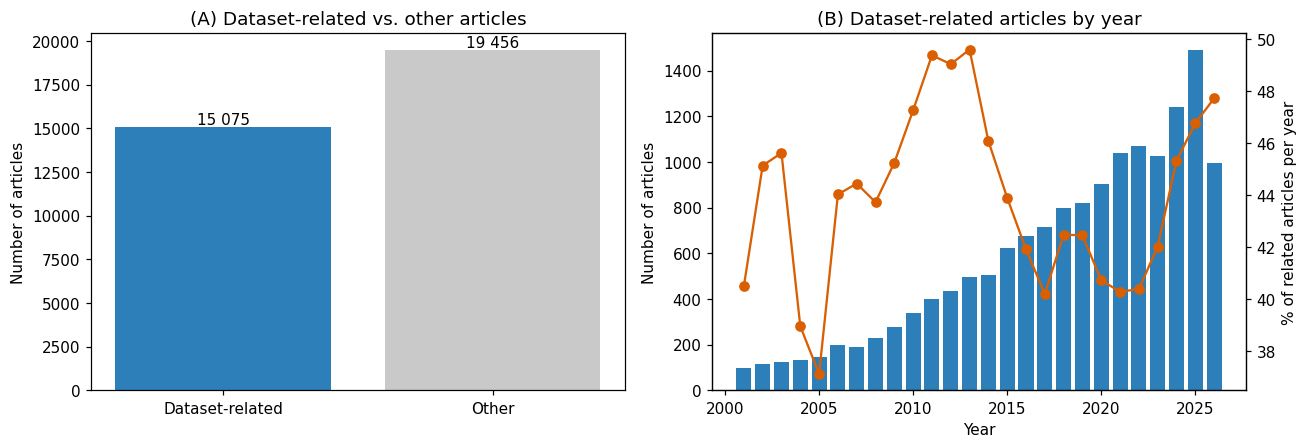
\includegraphics[width=\linewidth]{figs/task1_dataset_related.png}
%% Use \caption command for figure caption and label.
\caption{Number of published documents classified as dataset-related among 34 531 analysed documents (Panel A), and annual publication count of dataset-related articles with percentage of recognition based on title, abstract, and keyword analysis (Panel B).}\label{fig:dataset_related}
%% https://en.wikibooks.org/wiki/LaTeX/Importing_Graphics#Importing_external_graphics
\end{figure}



\subsection{Spatial Reference of Datasets}
\label{Review:sub3}

The geographic location of a dataset is a critical factor in data discovery and selection. In addition to data quality, spatial reference is among the most important attributes that researchers must evaluate when searching for relevant datasets. Using a vocabulary of canonical geographic terms (Table \ref{tab:detec_geo}), a spatial search was applied to titles and abstracts across all 34 531 documents. Of these, 23 023 documents mentioned a dataset location; 20 517 referenced a single country, 1 676 referenced a continental-scale area, and 830 referenced a global scope. A total of 11 508 documents (33.3\%) made no mention of geographic location in the title or abstract, a proportion that remained consistent across both dataset-related and all-document subsets (Figure \ref{fig:counry}). This finding reveals a systemic problem: even when datasets are discoverable and accessible, users may need to read through the full article and documentation to determine the spatial extent of the underlying data.
As an additional analysis, the spatial reference of datasets was cross-validated against the first-author institutional affiliation. In 20 368 documents with identifiable affiliation data, 75.4\% (15 347 out of 20 368) of datasets originated from the region associated with the first author's affiliation. The top contributors to the global dataset corpus were China, the USA, and India, followed by global and pan-European datasets, with Switzerland and Germany rounding out the top five country-level contributors (Figure \ref{fig:counry}, Panels A and B). This concentration of dataset creation in well-funded research economies raises important questions about the equitable distribution of scientific data infrastructure.

\begin{figure}[t]
\centering
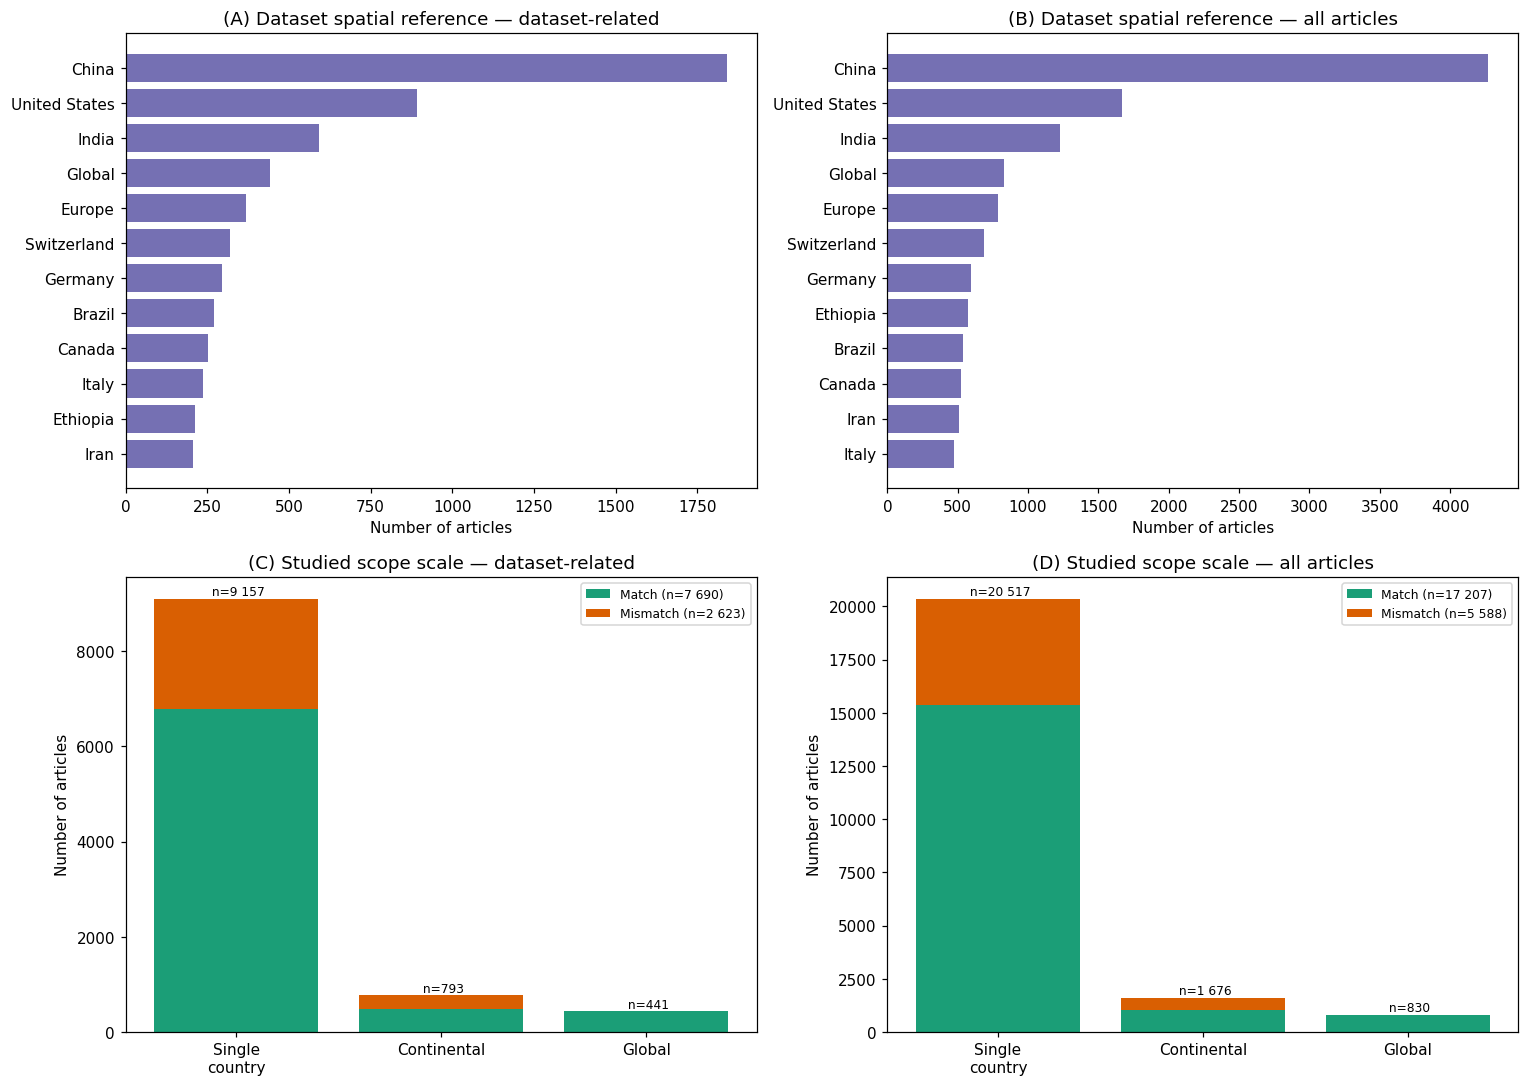
\includegraphics[width=\linewidth]{figs/task3_country_crossref.png}
\caption{Distribution of dataset repositories by country for dataset-related articles (Panel A) and all articles (Panel B), with spatial reference scope and mismatch between spatial reference and first-author affiliation for dataset-related (Panel C) and all articles (Panel D).}
\label{fig:counry}

\end{figure}

In Farmwise API framework  for all available and integrated dataset with allocation is already provided by the GUI where users can select a spatial reference and for this location dataset will be prepared. In addition on Github repository \citep{Smolak2025}. There is a unified and structure documentation of origin of dataset repository. 

\begin{table}[!ht]
    \centering
    \begin{tabularx}{\linewidth}{|l|X|}
    \hline
        \textbf{Canonical Category} & \textbf{Match Terms} \\ \hline
        Global & global, globally, worldwide, world-wide, world wide, across the world, \newline around the world, global scale, global-scale, planetary, all continents, multi-continental \\ \hline
        Multi-country & multi-country, multiple countries, cross-country, trans-national, \newline transnational, pan-tropical, pantropical, international \\ \hline
        Europe & europe, european, pan-european, continental europe, central europe, \newline eastern europe, western europe, northern europe, southern europe, european union \\ \hline
        Asia & asia, asian, south asia, southeast asia, south-east asia, east asia, \newline central asia, west asia, asia-pacific, asia pacific, indian subcontinent \\ \hline
        Africa & africa, african, sub-saharan africa, sub saharan africa, west africa, \newline east africa, north africa, southern africa, central africa, sahel, horn of africa, maghreb \\ \hline
        North America & north america, north american, central america, mesoamerica, caribbean, \newline the caribbean \\ \hline
        South America & south america, south american, latin america, latin american, andes, \newline andean, amazon basin, amazonia, the amazon, southern cone \\ \hline
        Oceania & oceania, australasia, pacific islands, polynesia, melanesia, micronesia \\ \hline
        Antarctica & antarctica, antarctic \\ \hline
    \end{tabularx}
    \caption{Vocabulary used to detect geographic terms for global, multi-country, and continental spatial reference in document titles and abstracts.}
    \label{tab:detec_geo}
\end{table}




\subsection{Type and Format of Published Datasets}
\label{Review:sub4}

From 2001 to 2026, the diversity of data formats and storage technologies has expanded substantially, in parallel with the development of Geographic Information Systems (GIS) and geospatial processing tools. Spatial datasets have become increasingly prevalent, offering visually interpretable representations of environmental processes and spatial relationships. A side effect of this proliferation has been the emergence of diverse coordinate reference systems, data formats of varying cross-community compatibility, and a wide range of spatial resolutions driven by developments in UAV and satellite remote sensing technology.
Among the collected documents, 60.2\% (20 784 out of 34 531) contained identifiable dataset format information in the title, abstract, or keywords. Agricultural datasets are dominated by spatial data types, with raster, remote sensing, geospatial, and image datasets accounting for 15 147 out of 20 784 identifiable records (Figure \ref{fig:data_format}). In-situ measurements, while less frequently published as standalone datasets, play an essential validation role for spatial products, particularly given the confounding effects of variables such as air humidity, cloud cover, and vegetation phenological stage on remote sensing retrievals. This validation gap is partly addressed by national meteorological offices, many of which continuously collect, process, and publish in-situ time-series data. The FARMWISE-API framework incorporates several such national meteorological office datasets.

\begin{figure}
\centering
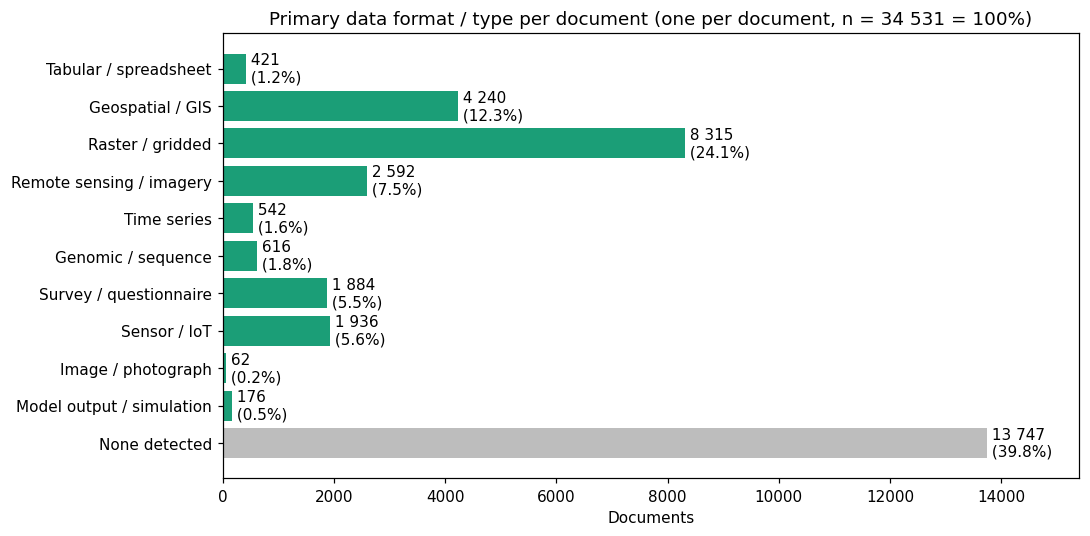
\includegraphics[width=\linewidth]{figs/task5_data_formats_primary.png}
\caption{Distribution of data formats and types identified in the reviewed dataset-related documents}
\label{fig:data_format}

\end{figure}


\section{Methodology: The FARMWISE-API Architecture}

\label{Methodology}

The user interface is built using the FastAPI framework and operates on a Uvicorn server configured with four worker processes, enabling concurrent request handling. The application provides three groups of endpoints organized into separate routers: (i) the main router, responsible for receiving requests for environmental data and forwarding them to the orchestration layer; (ii) a user authorization router, with user data stored in a relational database managed by SQLAlchemy; and (iii) a web interface router providing static resources. The application implements the FastAPI lifespan pattern for lifecycle management: upon startup, a temporary directory for output files is created and a job scheduler is launched; upon shutdown, the temporary directory is deleted.
The central component of the system is an asynchronous query dispatcher function that routes requests to appropriate data sources. The key mechanism of the dispatcher is iteration through a data source registry, performing a ternary coverage check for each registered source: (i) spatial coverage—whether the API's geographic coverage includes the desired area; (ii) temporal coverage—whether the data time range includes the desired period; and (iii) thematic coverage—whether the API provides at least one of the requested variables. Only sources that satisfy all three conditions are queried, eliminating unnecessary network requests before they are initiated. Requests to individual APIs are processed asynchronously with a configurable timeout (600 seconds by default), which prevents a single slow source from blocking the entire pipeline. Errors from individual adapters are logged without interrupting the processing of other sources.
FARMWISE-API framework have a build in interactive map tool was developed in the Python programming language. The following Python packages were used to create the interactive maps: pandas, numpy, s2sphere, shapely, rasterio, folium, io, PIL, base64, and branca.colormap \citep{foliumteam2025,Gillies2025,pandasdevelopmentteam2024,Rougier2015,s2spheredevelopmentteam2025, Rasteriodevelopmentteam2025,PythonTeam2025}. The interactive map is a standalone HTML file, meaning that once it is generated, it does not require any external datasets to function and can be freely shared.

\subsection{The wrapper layer—API modules}
\label{Meth:sub1}

Each external data source is represented by a separate Python module, loaded dynamically at runtime. This approach implements the Adapter design pattern: each module wraps the specific interface of an external API into a common call signature, decoupling the higher layers of the system from the implementation details of individual data providers 

\begin{figure}
\centering
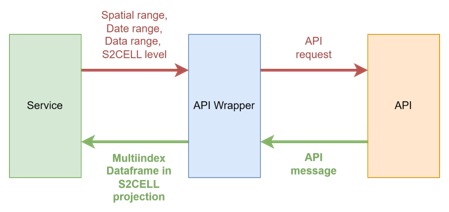
\includegraphics[width=\linewidth]{figs/obrazek_dominika.png}
\caption{Data flow in the adapter (wrapper) layer, illustrating how heterogeneous external APIs are mapped to a common internal interface.}
\label{fig:flow_chart}
\end{figure}


The system's central registry is a dictionary of adapters, storing three sets of ranges for each adapter: spatial, temporal, and thematic. This allows the dispatcher to efficiently filter sources without establishing network connections. Supported environmental variable categories include, among others, temperature, precipitation, potential evapotranspiration, soil properties, surface and groundwater resources, and land cover.
The hierarchical S2Cell grid, based on the Google S2 Geometry library \citep{s2spheredevelopmentteam2025}, was adopted as the system's common spatial reference framework. The S2 system divides the Earth's surface into a hierarchical mosaic of spherical quadrilaterals indexed by a Hilbert curve, ensuring efficient spatial indexing while preserving the locality of references. S2 cell identifiers are encoded as 64-bit integers, making them exceptionally efficient in big-data contexts. As demonstrated by \cite{Stephen2024}, Discrete Global Grid Systems (DGGS), to which S2 belongs, constitute a natural nexus for the integration and querying of heterogeneous geospatial data from multiple sources—a key property for the FARMWISE-API framework. The level parameter in a query specifies the grid resolution (ranging from coarse planetary-scale divisions to areas on the order of square metres), allowing users to flexibly control the spatial resolution of the output. Data returned by adapters takes the form of pandas DataFrame objects with a multi-level column index: the first level contains the variable name, and the second level contains the S2Cell identifier.

\subsection{Harmonization and Merging of Results}
\label{Meth:sub1}

After collecting responses from all matched sources, the dispatcher performs the following processing steps: (i) merging all DataFrames; (ii) averaging values from different sources for the same variables and cells; (iii) optional spatial interpolation of missing values; and (iv) optional generation of an interactive Folium map as an HTML file. Along with the data, metadata for each API call is returned: source name, available variables, covered date range, actual bounding box of the returned data, and call status. This metadata forms the basis for data quality assessment.

\section{Outputs of FARMWISE API - Exemplary results}
\label{Results}

TBD



\section{Discussion}
\label{Discussion}
The digital agricultural landscape is populated by a variety of platforms and initiatives, each with distinct strengths and limitations. A comparative analysis reveals a clear gap in the existing ecosystem that FARMWISE-API is designed to address.
Platforms such as the Water Information System for Europe (WISE) and the Copernicus Data Space Ecosystem \citep{Kovcs2026,WISE2026} provide a vast amount of public data free of charge. WISE serves as a gateway to water-related information collected by the European Commission and the European Environment Agency (EEA), covering themes such as water quality and contamination \citep{EEA2025,Commission2022,commission2025}. Similarly, Copernicus offers a comprehensive catalog of satellite imagery and climate, land, and marine data. The primary strength of these portals is their breadth of coverage and accessibility. However, their principal limitation is the provision of raw, unprocessed data, which requires significant technical expertise—including knowledge of programming and geospatial libraries—to process, analyse, and fuse across multiple disparate sources. The openEO API\citep{Schramm2021}, an open-source standard, partially addresses this by simplifying the processing of Earth observation data, but it remains primarily focused on satellite data and does not readily integrate with non-Earth observation streams.
The private sector has responded with specialized solutions. Weenat focuses on hyper-local agro-weather data, using a network of sensors and a proprietary algorithm to provide high-resolution temperature, precipitation, and soil moisture data \citep{Weenat2026}. Its strength lies in precision and interface simplicity; however, its scope is limited to a narrow set of data types, and its subscription-based commercial model constrains accessibility. Similarly, Agricolus is a precision farming platform that provides monitoring, pest management support, and decision tools, but prioritizes a full-service commercial platform over a generalized data fusion API for researchers and developers \citep{Agricolus2026}.
Agdatahub is a data intermediation platform providing a secure framework for data exchange between agri-food stakeholders, with its core value lying in ensuring data sovereignty. While it facilitates data movement, it is not a data fusion engine. The FaST Platform, supported by the European Commission, is designed to support farmers with administrative tasks and Common Agricultural Policy (CAP) compliance, integrating Copernicus satellite data; however, its primary function is regulatory rather than scientific data fusion.
This comparative landscape reveals that FARMWISE-API occupies a critical and largely unoccupied niche. Its core contribution lies not in being a new data source or regulatory platform, but in serving as a value-added integration engine. While other tools provide raw data (Copernicus, WISE) or specialized data services (Weenat), FARMWISE-API is built from the ground up to fuse disparate streams into a coherent, actionable product. This fusion-oriented architecture makes it an ideal tool for researchers and large-scale analytical projects requiring a holistic view of the agricultural system. Its open-science approach, which prioritizes reproducibility and standardization, positions it as a foundational layer for a new generation of decision support systems.
Nevertheless, FARMWISE-API faces clear challenges. Its value is entirely contingent on the availability and reliability of external APIs it consumes, creating a dependency on third-party services that may change, become unavailable, or alter their licensing conditions. Furthermore, the framework must navigate issues of data ownership and user privacy to earn the trust of farmers and other stakeholders. The business model—whether the framework will be maintained as a free, open-source public good or eventually monetized—requires careful deliberation to ensure long-term sustainability and widespread adoption.

\section{Conclusion}
\label{Conclusion}
FARMWISE-API is a direct and necessary response to the systemic problem of data fragmentation in European agriculture. This paper has demonstrated that while a vast amount of valuable data exists across public and private domains, its full potential is constrained by a lack of interoperability and common standards. The bibliometric analysis presented here confirms that more than half of relevant agricultural publications remain inaccessible behind paywalls, approximately one-third of dataset publications lack explicit spatial reference information, and the spatial distribution of dataset creation is strongly skewed towards well-funded research economies.
FARMWISE-API addresses these challenges by providing a unified data integration layer. By systematically collecting, standardizing, and synthesizing disparate meteorological and hydrological datasets from 19 sources across Europe, FARMWISE-API transforms raw heterogeneous data into a coherent and scientifically valuable resource. Its primary contribution is its fusion-oriented architecture: unlike public portals that offer raw data, commercial platforms with narrow scope, or data hubs that act as intermediaries, FARMWISE-API performs the complex, non-trivial function of combining data streams—a capability essential for generating the deep, actionable insights required for modern, sustainable agriculture.
The existence of integrated tools like FARMWISE-API represents not merely a technological advancement but a critical step towards building the digital infrastructure for a sustainable, resilient, and economically viable European agricultural sector. By making data findable, accessible, interoperable, and reusable, such platforms lay the foundation for a new era of evidence-based policy and practice, empowering stakeholders from individual farmers to EU policymakers to make better-informed decisions, ultimately supporting food security and environmental protection.
Future work should focus on several priority areas. First, the data ingestion layer could be expanded to include additional data streams such as soil quality indices and agricultural commodity market prices, to provide a more comprehensive picture. Second, while the current architecture is well-suited for researchers and developers, the development of a simplified user-facing decision support system (DSS) would make the platform's insights directly accessible to non-technical stakeholders. Finally, to address the critical issue of data trust and sovereignty, the platform should implement robust data governance protocols—including a consent management system—to align with evolving EU data legislation, including the Data Act.



\section{Acknowledgments}
\label{Ack}
The research was funded from the European Union’s Horizon Europe research and innovation programme under Grant Agreement number: 101135533

%% The Appendices part is started with the command \appendix;
%% appendix sections are then done as normal sections
\appendix
\section{Dataset Search Keywords}
\label{app:keywords}
The dictionary of 40 dataset-related terms used for article screening includes: \textit{dataset}, \textit{data set}, \textit{data-set}, \textit{datasets}, \textit{database}, \textit{data base}, \textit{data repository}, \textit{data archive}, \textit{data collection}, \textit{data product}, \textit{benchmark data}, \textit{open data}, \textit{data portal}, \textit{data record}, \textit{data descriptor}, \textit{remote sensing}, \textit{satellite imagery}, \textit{time series}, \textit{geospatial data}, \textit{gridded data}, \textit{reanalysis}, \textit{field survey}, \textit{monitoring network}, \textit{in situ measurements}, \textit{sensor data}, \textit{spatial data}, \textit{land cover}, \textit{land use}, \textit{inventory}, \textit{census}, \textit{spectral library}, \textit{training data}, \textit{labeled data}, \textit{annotated data}, \textit{raster}, \textit{shapefile}, \textit{geotiff}, \textit{data availability}, \textit{publicly available data}, and \textit{data sharing}.

\appendix
\section{Integrated Data Repositories}
\label{sec:appendix_repositories}

\begin{sidewaystable*}
    \centering
    \small
    \setlength{\tabcolsep}{5pt}
    \begin{tabularx}{\textwidth}{@{} >{\raggedright\arraybackslash}X l >{\raggedright\arraybackslash}X c c c @{}}
    \toprule
        \textbf{Repository name} & \textbf{Area covered} & \textbf{Type of data} & \textbf{Temporal coverage} & \textbf{Spatial resolution} & \textbf{Temporal resolution} \\ \midrule
        GIOS API – soil chemistry & Poland & Soil data & 1995-01-01 – 2020-12-31 & point-based & yearly (irregular) \\
        GIOS\_gw & Poland & GW quality, GW quantity & 1991-01-01 – 2023-12-31 & point-based & daily \\
        State Agency of Water Resources of Ukraine & Ukraine & SW quality & 1950-01-01 – current day & point-based & monthly \\
        Environmental Protection Agency of Ireland & Ireland & GW quantity & 1970-01-01 – current day & point-based & daily \\
        IMGW API – synop daily & Poland & Precipitation, Temperature & 1960-01-01 – current day & point-based & daily \\
        IMGW API – hydro daily & Poland & Hydrological data & 1951-01-01 – current day & point-based & daily \\
        ERA5 & Global & Meteorological data & 1950-01-01 – current day & grid-based & daily \\
        EGDI (European Geological Data Infrastructure) & Europe & Hydraulic conductivity & 1950-01-01 – current day & grid-based & daily \\
        EGDI (European Geological Data Infrastructure) & Europe & GW quantity & 1950-01-01 – current day & grid-based & daily \\
        DWD\_precipitation & Germany & Precipitation & 1950-01-01 – current day & point-based & daily \\
        DWD\_temperature & Germany & Temperature & 1950-01-01 – current day & point-based & daily \\
        Geosphere & Austria & Precipitation, Temperature & 1950-01-01 – current day & point-based & — \\
        Soil Grids & Europe & Soil data & 1951-01-01 – current day & grid-based & — \\
        Corine & Europe & Land cover & 1990-01-01 – current day & grid-based & none \\
        ADES (via Hub'Eau APIs) & France & GW quantity & 1950-01-01 – current day & point-based & daily \\
        ADES (via Hub'Eau APIs) & France & GW quality & 1969-01-01 – current day & point-based & daily \\
        Naïades (via Hub'Eau APIs) & France & SW quality & 1987-01-01 – current day & point-based & irregular \\
        EEA & Europe & Land cover & 2018-01-01 – current day & grid-based & — \\
        IFSGRID & Europe & Livestock pressure, SW quality, land cover, agricultural structure & 2020-01-01 – current day & grid-based & — \\ \bottomrule
    \end{tabularx}
    \caption{Complete overview of repositories integrated within the FARMWISE-API framework, including coverage area, data type, temporal coverage, spatial resolution, and temporal resolution.}
    \label{tab:repo_appendix_complete}
\end{sidewaystable*}

%% If you have bib database file and want bibtex to generate the
%% bibitems, please use
%%
\bibliographystyle{elsarticle-harv} 
\bibliography{FARMWISTE_API_dt}

%% else use the following coding to input the bibitems directly in the
%% TeX file.

%% Refer following link for more details about bibliography and citations.
%% https://en.wikibooks.org/wiki/LaTeX/Bibliography_Management

%%\begin{thebibliography}{00}

%% For authoryear reference style
%% \bibitem[Author(year)]{label}
%% Text of bibliographic item

%%\end{thebibliography}


\end{document}

\endinput
%%
%% End of file `elsarticle-template-harv.tex'.


